\documentclass{beamer}
\usetheme{Boadilla} % Pretty neat, soft color.
\setbeamercovered{invisible}
\setbeamertemplate{navigation symbols}{}
\setbeamertemplate{caption}[numbered]

% contains all commands, package imports 
\usepackage{blubase}
\usepackage{multicol}
\usepackage{thmtools}
% theorem environments
\theoremstyle{plain}
\newtheorem{proposition}[theorem]{Proposition}
\newtheorem{conjecture}[theorem]{Conjecture}
\newtheorem{question}[theorem]{Question}
\declaretheorem[style=plain, name = Definition,numbered=no]{definition*}

\usepackage{tikz}
\newcommand*\circled[1]{\tikz[baseline=(char.base)]{
\node[shape=circle,draw,inner sep=1pt] (char) {#1};}}

\renewcommand{\mod}[2]{\equiv#1\ \left(\textup{mod }#2\right)}

\xdefinecolor{dred}{RGB}{90,0,0}
\xdefinecolor{lred}{RGB}{255,240,230}
\setbeamercolor{upperr}{fg=white,bg=dred}
\setbeamercolor{lowerr}{fg=black,bg=lred}
\xdefinecolor{dgreen}{RGB}{0,90,0}
\xdefinecolor{lgreen}{RGB}{240,255,230}
\setbeamercolor{upperg}{fg=white,bg=dgreen}
\setbeamercolor{lowerg}{fg=black,bg=lgreen}

%\newcolumntype{M}[1]{>{\centering\arraybackslash}m{#1}}
\newcolumntype{N}{@{}m{0pt}@{}}

\makeatletter
\newcommand{\thickhline}{\noalign {\ifnum 0=`}\fi \hrule height 1pt \futurelet \reserved@a \@xhline}

\def\msquare{\mathord{\scalerel*{\Box}{gX}}}

\title[]{What's Next? \\ {\normalsize math stories from beyond VMT}}
\author{Bryan Lu}
\date{June 5, 2023}

\begin{document}

\begin{frame}
\begin{center}
  {\Large \tbf{Question.} What does math/doing math mean to you?} 
 \begin{multicols}{2}
    \begin{itemize}
      \item Why do you want to study math?
      \item Do you like math? Why?
      \item How could you learn about math outside of school/VMT?
      \item What does being ``good'' at math mean?
      \item How diverse is the math community?
      \item Does doing math make you ``smarter?''
      \item Why should people study math?
    \end{itemize}
  \end{multicols}
\end{center}
\end{frame}

\begin{frame}
\titlepage
\end{frame}

\usebackgroundtemplate{ }

\begin{frame}{Your Landscape}
  \begin{center}
    \begin{minipage}{0.45\textwidth}
      Competition math categories:
      \begin{itemize}
        \item algebra (inequalities, FEs)
        \item geometry (mostly Euclidean)
        \item combinatorics
        \item number theory (elementary)
      \end{itemize}
    \end{minipage}
    \pause
    \begin{minipage}{0.45\textwidth}
      TJ Math (engineering reqs):
      \begin{itemize}
        \item calculus (BC + multi)
        \item linear algebra 
        \item differential equations 
        \item statistics  
      \end{itemize}            
    \end{minipage}        
  \end{center} 
  \pause
 This is \tbf{VERY FAR} from everything that's out there!
\end{frame}

\begin{frame}{Further Fields of Study}
  Typical undergraduate categories: 
  \begin{center}
    \begin{minipage}{0.45\textwidth}
      Main categories of study:
      \begin{itemize}
        \item (abstract) algebra       
        \item analysis/measure                           
       \item topology/geometry
      \end{itemize}
    \end{minipage}
    \pause
  \begin{minipage}{0.45\textwidth}
   Less central categories:
    \begin{itemize}
      \item combinatorics
      \item logic/set theory
      \item probability/statistics
    \end{itemize} 
  \end{minipage}
  \end{center}
  \pause
  Broader fields (incomplete/ill-defined list; historically important): 
  \begin{center}
   \begin{multicols}{3}
    \begin{itemize}
      \item algebraic number theory
      \item analytic number theory
      \item dynamical systems
      \item Lie theory
      \item harmonic analysis
      \item operator theory
      \item computer science
      \item foundations
      \item game theory/economics
      \item algebraic geometry
      \item algebraic topology
      \item mathematical physics 
    \end{itemize}
  \end{multicols} 
  \end{center}
\end{frame}

\begin{frame}{Dependency Graph (\tit{Napkin, Evan Chen})}
  \begin{center}
    \includegraphics[width=\textwidth]{recent-flowchart-napkin.png}
  \end{center}  
\end{frame}

\begin{frame}{Myths/Misconceptions}
 \begin{enumerate}
  \item Proving really \tbf{hard} theorems/solving really \tbf{hard} problems
    (misplaced emphasis) 
   \pause
  \item Formalism vs. pedantry
   \pause
  \item Working on your own vs. community of ideas
   \pause
  \item Difficulty as a barrier to growth
   \pause
  \item (there are probably tons more \dots)  
\end{enumerate} 
\end{frame}

\begin{frame}{Core Ideas}
 \begin{enumerate}
  \item Connecting seemingly unrelated objects/procedures.  
   \pause
  \item Extending/generalizing ideas we already know. 
   \pause
  \item Analyzing when/why patterns break and seeking complexity.
   \pause
  \item Staying grounded with ``standard'' examples/calculations. 
\end{enumerate} 
\end{frame}

\begin{frame}{the rest of this lecture: choose your own adventure}
 \begin{itemize}
   \item for each Core Idea I present two fields of study that I
     think exemplify this idea
    \pause
   \item read the descriptions of what I would talk to you about for each 
     field of study I've selected
     -- \tit{a star means a subject is less accessible}
    \pause
    \item crowd vote!! \pause $\Rightarrow$ this talk could go in 8 possible ways
 \end{itemize} 
\end{frame}

\begin{frame}{Idea 1 -- Connections}
 \begin{itemize}
   \item \textit{How to Tell Spaces Apart (Simplicial Homology)} --
    We will use graphs as a model for describing various topological spaces
    (spheres, toruses, Klein bottles) and use an extension of the Euler
    characteristic with linear algebra to distinguish spaces from each other. 
  \item ($\bigstar$) \tit{Word Problems (Geometric Group Theory)} -- We
    will take an alternate view of groups and study graphs induced by a group's
    structure, and use these graphs to explain why deciding whether an element
    in a group is the identity element is unsolvable.  
 \end{itemize} 
\end{frame}

\begin{frame}{1.1 -- Euler Characteristic}
 Euler characteristic of a graph $G$ with $V$ vertices, $E$ edges,
 and $F$ faces: $\chi(G) = V - E + F$.
\begin{center}
 \begin{tikzpicture}
        \draw[fill=gray!30] (0,0) -- ++(3,0) -- ++(0, 3) -- ++(-3,-3) ;
       \node[circle,inner sep=1pt](D) at (2,1) {$B$};
       \draw[fill=gray!15] (0,0) -- ++(0,3) -- ++(3, 0) -- ++(-3,-3) ;
       \node[circle,inner sep=1pt](U) at (1,2) {$A$};
       \node[circle,fill,inner sep=1pt,label=below:$v_1$](p00) at (0,0) {};
       \node[circle,fill,inner sep=1pt,label=below:$v_2$](p10) at (3,0) {};
       \node[circle,fill,inner sep=1pt,label=above:$v_4$](p01) at (0,3) {};
       \node[circle,fill,inner sep=1pt,label=above:$v_3$](p11) at (3,3) {};

      \draw (p00) -- node[midway, above, left] {$g$} (p11);
      \draw (p00)  -- node[midway, below] {$e_1$} (p10) ;
      \draw (p01)  -- node[midway, above] {$e_2$} (p11) ;
      \draw (p00)  -- node[midway, left] {$f_1$} (p01) ;
      \draw (p10)  -- node[midway, right] {$f_2$} (p11) ;
    \end{tikzpicture}

    $\chi(G) = 2$
\end{center}
\end{frame}

\begin{frame}{1.1 -- Example Spaces}
 \begin{center}
    \begin{tikzpicture}
        \draw[fill=gray!30] (0,0) -- ++(2,0) -- ++(0, 2) -- ++(-2,-2) ;
       \node[circle,inner sep=1pt](D) at (1.5,0.5) {$B$};
       \draw[fill=gray!15] (0,0) -- ++(0,2) -- ++(2, 0) -- ++(-2,-2) ;
       \node[circle,inner sep=1pt](U) at (0.5,1.5) {$A$};
       \node[circle,fill,inner sep=1pt,label=below:$v_1$](p00) at (0,0) {};
       \node[circle,fill,inner sep=1pt,label=below:$v_2$](p10) at (2,0) {};
       \node[circle,fill,inner sep=1pt,label=above:$v_2$](p01) at (0,2) {};
       \node[circle,fill,inner sep=1pt,label=above:$v_3$](p11) at (2,2) {};

      \draw[-{Stealth[length=3mm, width=2mm]}, purple] (p00) -- node[midway, above, left] {$g$} (p11);
      \draw[-{Stealth[length=3mm, width=2mm]}, red] (p00)  -- node[midway, below] {$e$} (p10) ;
      \draw[-{Stealth[length=3mm, width=2mm]}, blue] (p01)  -- node[midway, above] {$f$} (p11) ;
      \draw[-{Stealth[length=3mm, width=2mm]}, red] (p00)  -- node[midway, left] {$e$} (p01) ;
      \draw[-{Stealth[length=3mm, width=2mm]}, blue] (p10)  -- node[midway, right] {$f$} (p11) ;
    \end{tikzpicture}
    \begin{tikzpicture}
        \draw[fill=gray!30] (0,0) -- ++(2,0) -- ++(0, 2) -- ++(-2,-2) ;
       \node[circle,inner sep=1pt](D) at (1.5,0.5) {$B$};
       \draw[fill=gray!15] (0,0) -- ++(0,2) -- ++(2, 0) -- ++(-2,-2) ;
       \node[circle,inner sep=1pt](U) at (0.5,1.5) {$A$};
       \node[circle,fill,inner sep=1pt,label=below:$v$](p00) at (0,0) {};
       \node[circle,fill,inner sep=1pt,label=below:$v$](p10) at (2,0) {};
       \node[circle,fill,inner sep=1pt,label=above:$v$](p01) at (0,2) {};
       \node[circle,fill,inner sep=1pt,label=above:$v$](p11) at (2,2) {};

      \draw[-{Stealth[length=3mm, width=2mm]}, purple] (p00) -- node[midway, above, left] {$g$} (p11);
      \draw[-{Stealth[length=3mm, width=2mm]}, red] (p00)  -- node[midway, below] {$e$} (p10) ;
      \draw[-{Stealth[length=3mm, width=2mm]}, red] (p01)  -- node[midway, above] {$e$} (p11) ;
      \draw[-{Stealth[length=3mm, width=2mm]}, blue] (p00)  -- node[midway, left] {$f$} (p01) ;
      \draw[-{Stealth[length=3mm, width=2mm]}, blue] (p10)  -- node[midway, right] {$f$} (p11) ;
    \end{tikzpicture}
\end{center}
\begin{center}
    \begin{tikzpicture}
        \draw[fill=gray!30] (0,0) -- ++(2,0) -- ++(0, 2) -- ++(-2,-2) ;
       \node[circle,inner sep=1pt](D) at (1.5,0.5) {$B$};
       \draw[fill=gray!15] (0,0) -- ++(0,2) -- ++(2, 0) -- ++(-2,-2) ;
       \node[circle,inner sep=1pt](U) at (0.5,1.5) {$A$};
       \node[circle,fill,inner sep=1pt,label=below:$v_2$](p00) at (0,0) {};
       \node[circle,fill,inner sep=1pt,label=below:$v_1$](p10) at (2,0) {};
       \node[circle,fill,inner sep=1pt,label=above:$v_1$](p01) at (0,2) {};
       \node[circle,fill,inner sep=1pt,label=above:$v_2$](p11) at (2,2) {};

      \draw[-{Stealth[length=3mm, width=2mm]}, purple] (p00) -- node[midway, above, left] {$g$} (p11);
      \draw[{Stealth[length=3mm, width=2mm]}-, red] (p00)  -- node[midway, below] {$e$} (p10) ;
      \draw[-{Stealth[length=3mm, width=2mm]}, red] (p01)  -- node[midway, above] {$e$} (p11) ;
      \draw[{Stealth[length=3mm, width=2mm]}-, blue] (p00)  -- node[midway, left] {$f$} (p01) ;
      \draw[-{Stealth[length=3mm, width=2mm]}, blue] (p10)  -- node[midway, right] {$f$} (p11) ;
    \end{tikzpicture}
    \begin{tikzpicture}
        \draw[fill=gray!30] (0,0) -- ++(2,0) -- ++(0, 2) -- ++(-2,-2) ;
       \node[circle,inner sep=1pt](D) at (1.5,0.5) {$B$};
       \draw[fill=gray!15] (0,0) -- ++(0,2) -- ++(2, 0) -- ++(-2,-2) ;
       \node[circle,inner sep=1pt](U) at (0.5,1.5) {$A$};
       \node[circle,fill,inner sep=1pt,label=below:$v$](p00) at (0,0) {};
       \node[circle,fill,inner sep=1pt,label=below:$v$](p10) at (2,0) {};
       \node[circle,fill,inner sep=1pt,label=above:$v$](p01) at (0,2) {};
       \node[circle,fill,inner sep=1pt,label=above:$v$](p11) at (2,2) {};

      \draw[-{Stealth[length=3mm, width=2mm]}, purple] (p00) -- node[midway, above, left] {$g$} (p11);
      \draw[-{Stealth[length=3mm, width=2mm]}, red] (p00)  -- node[midway, below] {$e$} (p10) ;
      \draw[-{Stealth[length=3mm, width=2mm]}, red] (p01)  -- node[midway, above] {$e$} (p11) ;
      \draw[-{Stealth[length=3mm, width=2mm]}, blue] (p00)  -- node[midway, left] {$f$} (p01) ;
      \draw[{Stealth[length=3mm, width=2mm]}-, blue] (p10)  -- node[midway, right] {$f$} (p11) ;
    \end{tikzpicture}
  
\end{center} 
\end{frame}

\begin{frame}{1.1 -- Chain Complexes}
\[\sigma = [v_0, v_1, \dots, v_n]\]
  \[
  \Rightarrow \bound \sigma = \sum_{i=0}^n (-1)^i \sigma\big|_{[v_0, v_1, \dots, v_{i-1},
v_{i+1}, \dots, v_n]}
  \]
  \pause
  \[
  \dots \to C_n(G) \xto {\partial_n} \dots \to C_2(G) \xto{\partial_2} C_1(G)
  \xto{\partial_1} C_0(G) \xto{\partial_0} 0  
\]
\centering \tit{Holes have no boundary, but are not the boundary of any
simplex.}
\[
  \boxed{\bound^2 = 0} \pause \Rightarrow \boxed{H_n(G) = \frac{\phantom{\ker} \bound_{\phantom n}}{\phantom{\im}
  \bound_{\phantom{n+1}}}} 
\]
\end{frame}

\begin{frame}{1.1 -- Homology Groups}
  \begin{center}
    \begin{tabular}{c|ccccc}
      $G$ & $S^2$ & $\TT^2$ & $\RR P^2$ & $K$ \\ \hline
      $H_0(G)$ & $\ZZ$ & $\ZZ$ & $\ZZ$ & $\ZZ$ \\ 
      $H_1(G)$ & $0$ & $\ZZ^2$ & $\ZZ / 2 \ZZ $ & $\ZZ \times \ZZ / 2\ZZ$ \\ 
      $H_2(G)$ & $\ZZ$ & $\ZZ$ & $0$ & $0$ \\ 
    \end{tabular}
\end{center}
\end{frame}

\begin{frame}{1.1 -- Identical Homology}
  \begin{center}
    $\TT^2$ \qquad \qquad $S^1 \vee S^1 \vee S^2$

    $H_0 = \ZZ$ \quad $H_1 = \ZZ^2$ \quad $H_2 = \ZZ$

    \vspace{5cm}
  \end{center}
\end{frame}

\begin{frame}{1.2 -- Presentations}
  \begin{center}
$G = \tuple{S \mid R}$

\pause
    $S$ -- set of symbols \quad $S^{-1}$ -- each symbol tagged with an
    inverse

    \pause
    $L(S \cup S^{-1})$ -- all strings in letters of $S \cup S^{-1}$
   
    \pause
    $R$ -- words $w \in L(S \cup S^{-1})$ in $S \cup S^{-1}$ equal to $e$

    \pause
    $x s s^{-1} y \sim x s^{-1} s y \sim xy \sim x r y$

    \pause
    $\tuple{S | R}$ is the set of equivalence classes of $L(S \cup S^{-1})$
    under $\sim$
    \pause

    \begin{multicols}{2}
      \begin{enumerate}
      \item $\tuple{a \mid }$ 
      \item $\tuple{a \mid a^n}$ 
      \item $\tuple{a, b \mid a^3, b^2, (ab)^2 }$
      \item $\tuple{a, b \mid aba^{-1}b^{-1}}$ 
      \item $\tuple{a, b \mid a^n, b^2, (ab)^2 }$
      \item $\tuple{a, b \mid a^2, b^2}$
    \end{enumerate}
    \end{multicols}
  \end{center}
\end{frame}

\begin{frame}{1.2 -- Cayley Graphs}
  \begin{definition*}
    The \tbf{Cayley graph} of a group $G = \tuple{S \mid R}$, $\cay(G)$, has
    vertices $g$ for every $g \in G$, and directed edges $g \to gs$. 
  \end{definition*}
  \begin{center}
    \pause
    \includegraphics[width=0.3\textwidth]{cayley-graph-Z.png}
    \pause\includegraphics[width=0.3\textwidth]{cayley-graph-Z_n.png}
    \pause
    \includegraphics[width=0.3\textwidth]{cayley-graph-S_3.png}
  \end{center}
\end{frame}

\begin{frame}{1.2 -- Cayley Graphs}
  \begin{definition*}
    The \tbf{Cayley graph} of a group $G = \tuple{S \mid R}$, $\cay(G)$, has
    vertices $g$ for every $g \in G$, and directed edges $g \to gs$. 
  \end{definition*}
  \begin{center}
    \pause
    \includegraphics[width=0.3\textwidth]{cayley-graph-Z2.png}
    \pause\includegraphics[width=0.3\textwidth]{cayley-graph-D_6.png}
    \pause\includegraphics[width=0.3\textwidth]{cayley-graph-Dinfinity.png}
  \end{center}
\end{frame}

\begin{frame}{1.2 -- The Word Problem}
  \begin{problem}[The Word Problem]
  Given a group $G$ with finite presentation $\tuple{S \mid R}$ (i.e. $S$ and
  $R$ are both finite), for any word $w \in L(S \cup S^{-1})$, decide
  whether $[w]$ is the identity element $e$ in a finite amount of time.   
\end{problem}
\begin{center}
  \includegraphics[width=0.4\textwidth]{cayley-graph-ex.png}
\end{center}
\end{frame}

\begin{frame}{1.2 -- Bad News}
  \begin{theorem}[Novikov-Boone]
  The word problem for finitely presented groups is \tbf{undecidable} -- in
  particular, there exists a finitely presented group $G$ for which the word
  problem is undecidable. 
\end{theorem}
\pause
  \begin{theorem}[Higman's Embedding Theorem]
  Every finitely generated, \tbf{recursively presented} group $H$ can be embedded as a
 subgroup of some finitely presented group $G$, i.e. $H$'s
 set of relations is \tbf{recursively enumerable}. 
\end{theorem}
\end{frame}

\begin{frame}{1.2 -- Free Groups}
 \[
   F_n = \tuple{x_1, \dots, x_n \mid }
 \]
 \begin{center}
   \includegraphics[width=0.4\textwidth]{cayley-graph-F_2.png} 
 \end{center}
 \pause
 \begin{theorem}[Nielson-Schreier]
   Every subgroup of a free group is free. 
 \end{theorem}
\end{frame}
\begin{frame}{Idea 2 -- Generalizations}
 \begin{itemize}
   \item $(\bigstar)$ \tit{Doing Calculus Anywhere (Manifolds,
    Differential Forms)} -- One of the staples of calculus is the Fundamental
    Theorem of Calculus, which has many further generalizations further afield
    in multivariable calculus. Let's see why these are actually all the same
    thing! 

  \item \tit{A Case Study in Volume (Measure Theory)} -- So you
    think you know what volume is? Here we test your intuitive understanding of
    volume and use edge cases as a case study for generalizing what you might
    think of as ``volume.'' 
 \end{itemize} 
\end{frame}

\begin{frame}{2.1 -- Fundamental Theorems of (Multivariable) Calculus}
\begin{theorem}[Fundamental Theorem of Calculus]
  \[
   \int_a^b f(x) \, dx = F(b) - F(a).
  \]  
\end{theorem}
\pause
  \begin{theorem}[Fund. Thm. of Line Integrals]
   \[
    \int_\gamma \grad \vphi(\vec r) \cdot d\vec r = \vphi(\gamma(1)) -
    \vphi(\gamma(0)).
   \] 
  \end{theorem} 
      \begin{theorem}[Green's Theorem]
     \[
      \oint_C (L \, dx + M \, dy) = \iint_D \left( \pdv M x - \pdv L y \right)
      \, dx \, dy
     \] 
   \end{theorem}
\end{frame}

\begin{frame}{2.1 -- Fundamental Theorems of (Multivariable) Calculus}
      \begin{theorem}[Kelvin-Stokes' Theorem]
        \[
      \iint_S (\curl \vec F) \cdot d\vec S = \oint_{\bound S} \vec F \cdot
      d\vec r
    \]
   \end{theorem}
   \begin{theorem}[Divergence Theorem]
     \[
      \iint_V (\div \vec F) \, d V = \oiint_{\bound V} \vec F \cdot d \vec S
     \] 
   \end{theorem}
   \pause
   \begin{center}
     What do these theorems all have in common?

     \tit{Integrating a \tbf{function} over the \tbf{boundary of a space}
     is equal to integrating the \tbf{derivative} over the \tbf{whole space}.}
   \end{center}
\end{frame}

\begin{frame}{2.1 -- Generalized Stokes' Theorem}
 \begin{theorem}[Generalized Stokes' Theorem]
  Let {\color{purple}$M$} be a $k$-dimensional \tbf{\color{blue} oriented} \tbf{\color{purple}
  smooth manifold-with-boundary} in $\RR^n$, and give the boundary
  {\color{purple}$\bound M$} the \tbf{\color{blue} boundary orientation}. Let
  {\color{orange}$\vphi$} be a smooth
  {\color{orange}$(k-1)$}\tbf{\color{orange}-form} defined on an open set
  containing $M$. Then 
  \[
    {\color{blue}\int_{\color{purple}\bound M} {\color{orange}\vphi}} =
    {\color{blue}\int_{\color{purple}
    M} {\color{red}\mathrm{d}} {\color{orange}\vphi}}.
  \] 
\end{theorem} 
\end{frame}

\begin{frame}{2.1 -- Example}
\begin{problem}
  Verify that Stokes' Theorem holds for the surface $S$ given by $z = 5 - x^2 -
  y^2$ above the plane $z = 1$ (oriented upwards), and vector field $\vec F =
  z^2 \hat i - 3xy \hat j + x^3 y^3 \hat k$. 
\end{problem} 

\begin{center}
  \includegraphics[width=0.7\textwidth]{surface-example.png}
\end{center}
\end{frame}


\begin{frame}{2.2 -- Warmups}
 I hear y'all know how to find volumes in geometry -- let's test that!
 
What's the volume of: 
 \begin{itemize}
\pause
   \item A three-dimensional ball of radius 1? $(\set{\vec
    x \in \RR^3 : |\vec x| \leq 1})$
  \pause
  \item A two-dimensional disk of radius 1? $(\set{\vec x \in \RR^2 : |\vec x|
    \leq 1})$
  \pause
  \item The interval $[0,1]$ in $\RR$?  
  \pause
  \item The singleton point $\set 0$?
 \end{itemize}
\end{frame}

\begin{frame}{2.2 -- Linear Exercises (Part I)}
  For the following, tell me whether the volume of the following sets are $0$,
  $1$, or not defined, in $\RR$: 
  \begin{enumerate}
    \pause
    \item The two points $\set{0, 1}$. 
  \pause
    \item For $n \in \ZZ^+$, $\set{\frac k n : 0 \leq k \leq n, k \in
    \ZZ}$ (fractions with denominator $n$).
\pause
  \item The converging sequence $\set{\frac 1 {2^k} : k \in \ZZ_{\geq 0}}$.
\pause
  \item All dyadic fractions between 0 and 1, $\set{\frac m {2^n} : m, n \in
    \ZZ} \cap [0,1]$ (fractions whose denominator is a power of 2). 
  \pause
  \item The rational numbers between $0$ and $1$, $\QQ \cap [0, 1]$.
  \end{enumerate}
\end{frame}

\begin{frame}{2.2 -- Linear Exercises (Part II)}
  For the following, tell me whether the volume of the following sets are $0$,
  $1$, or not defined: 
 
  \begin{enumerate}
    \setcounter{enumi}{5}
  \pause
  \item Let $C_0 = [0,1]$, and
    for $n \geq 1$, assuming $C_{n-1}$ is a disjoint union of closed intervals, 
    remove the middle third of each interval to get $C_n$. Let $C = \bigcap_{k=0}^\infty
    C_k$. (This set is \textit{uncountable},
    unlike any of the examples up until this point.)
\pause
  \item Let $F_0 =
    [0,2]$. To generate $F_1$, remove the middle $\frac{1}{4}$ of each closed
    interval in $F_0$. In general, remove the
    middle $\frac{1}{4^i}$ of each interval from the intervals in $F_{i-1}$
    to get $F_i$. Let $F = \bigcap_{k=0}^\infty F_k$. 
\pause
  \item Consider $[0,1]$ under the equivalence relation $\sim$ such that $x \sim
    y$ if $|x - y| \in \QQ$. Partition $[0,1]$ into equivalence classes, and let
    $V$ consist of one representative from each equivalence class.
  \end{enumerate}
\end{frame}

\begin{frame}{2.2 -- Dimension Warmups}
  Now, let's warm up for a different question:
   \begin{itemize}
      \pause\item What's the 1-D volume of the sphere of radius
        $\frac{1}{2\sqrt \pi}$ in $\RR^3$?
      \pause\item What's the 2-D volume of the sphere of radius
        $\frac{1}{2\sqrt \pi}$ in $\RR^3$?
      \pause\item What's the 3-D volume of the sphere of radius
        $\frac{1}{2\sqrt \pi}$ in $\RR^3$? 
   \end{itemize}
   \pause
  Note that for only one of these is the answer not $0$ or $\infty$ -- it's when
  the dimension is 2! We can actually define the dimension in this way...
\end{frame}

\begin{frame}{2.2 -- Dimensionality Exercises}
 For these spaces, compute the definition in this way, assuming there is some $d
 \in \RR^+$ for which the volume is positive and finite (it's not going to be
 integral!):
 \begin{enumerate}
     \item The Cantor set $C$. 
  \item The Sierpinski triangle.
  \item The Koch snowflake.
  \item The Menger sponge. 
    \begin{center}
      \includegraphics[width=0.3\textwidth]{koch.png}
      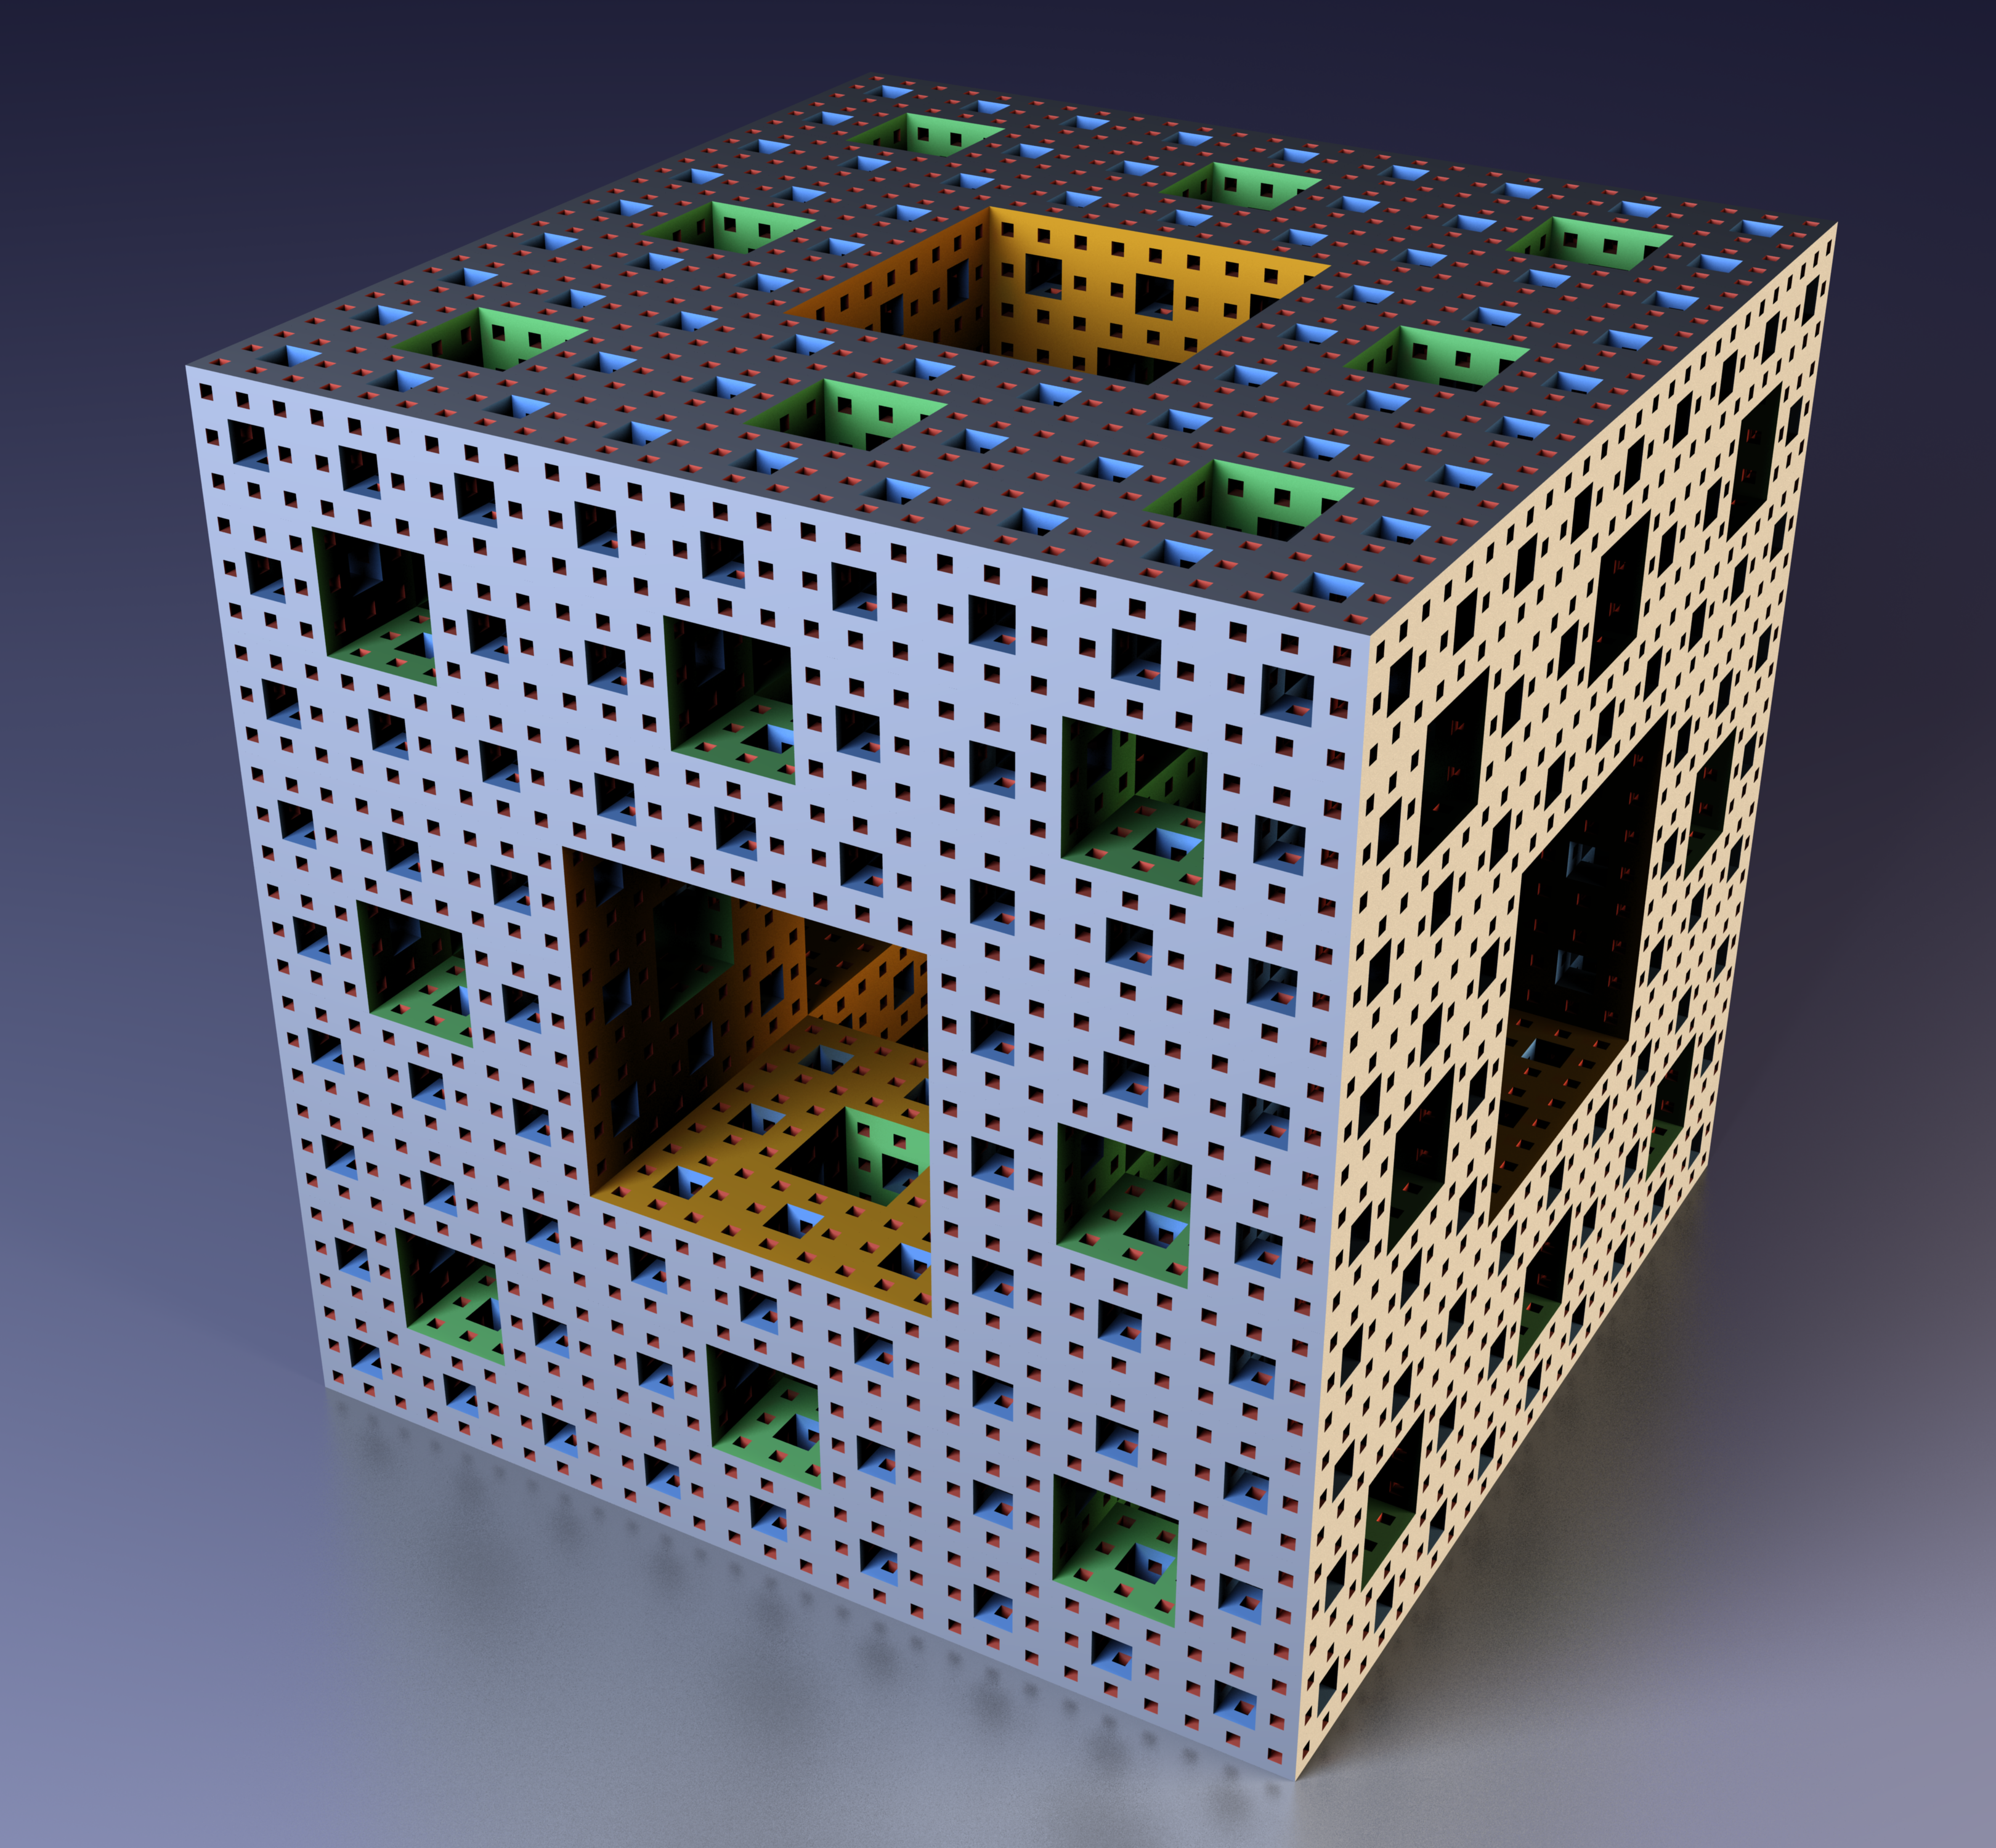
\includegraphics[width=0.3\textwidth]{menger.png}
    \end{center}
 \end{enumerate}
\end{frame}


\begin{frame}{Idea 3 -- Breaking and Repairing}
 \begin{itemize}
    \item \tit{I Forgot How to Factor (Algebraic
    Number Theory)} -- We will try solving some Diophantine equations in some
    creative ways, and realize that I don't really know how to prime-factorize
    things anymore. Can we fix that? 

  \item \tit{The Answer Is Not True (Analysis/Foundations)} -- Because everyone loves the true/false section of a math 
    exam, we're going to have a true/false party!

    Wait, I forgot to take the spoiler out of the section header... fine, to
    make it more interesting, be prepared to explain your answers!
 
 \end{itemize} 
\end{frame}

\begin{frame}{3.1 -- A Diophantine Equation}
 \begin{problem}
   Find all solutions in integers to $y^2 = x^3 - 1$. 
 \end{problem} 
\[
\pause \Rightarrow x^3 = y^2 + 1 \pause = (y+i)(y-i) 
\]
$y$ is not odd -- if it were, then $y^2 + 1 \equiv 2 \pmod 4$ and $x^3 \equiv 0
\pmod 4$. 
\pause
\noindent\tbf{Claim.} $y+i$ and $y-i$ have no non-unit common divisors.
\pause

\noindent\tit{Proof.} $\pi \mid y+i, y-i \Rightarrow \pi \mid 2i = (1+i)^2
\Rightarrow \pi = (1+i)$. \pause Then $y+i = (1+i)(a + bi), y-i = (1-i)(a-bi)
\Rightarrow y^2 + 1 = 2(a^2 + b^2)$. Contradiction, $y^2 + 1$ is odd.
\pause
\noindent $(y+i) = (a+bi)^3 = (a^3 - 3ab^2) + (3a^2b - b^3)$, so $b(3a^2 - b^2)
= 1$, and $b = \pm 1$. \pause If $b = 1$, no sol'ns, if $b = -1$, then $a = 0$,
so $y = 0$, $x = 1$. 

\pause $\Rightarrow (x,y) = (1, 0)$ is the only solution.
\end{frame}

\begin{frame}{3.1 -- Another Diophantine Equation}
 \begin{problem}
   Find all solutions in integers to $y^2 = x^3 - 61$. 
 \end{problem} 
\[
  \pause \Rightarrow x^3 = y^2 + 61 \pause = (y+\sqrt{-61})(y-\sqrt{-61}) 
\]
$y$ is not odd -- if it were, then $y^2 + 61 \equiv 2 \pmod 4$ and $x^3 \equiv 0
\pmod 4$. 
\pause
\noindent\tbf{Claim.} $y+\sqrt{-61}$ and $y-\sqrt{-61}$ have no non-unit common divisors.
\pause

\noindent\tit{Proof.} $\pi \mid y+\sqrt{-61}, y-\sqrt{-61} \Rightarrow \pi \mid
2\sqrt{-61}$. \pause $|\pi|^2 \mid y^2 + 61$ odd so $|\pi|^2$ odd, and therefore $|\pi|^2 =
61$. \pause Then $61 \mid y^2 + 61$, $61 \mid y$, and so $61 \mid x$ and so
$61^2 \mid x^3 - y^2 = 61$, contradiction. 
\pause
\noindent $(y+\sqrt{-61}) = (a+b\sqrt{-61})^3 = (a^3 - 183ab^2) + (3a^2b -
61b^3)$, so $b(3a^2 - 61b^2)
= 1$, and $b = \pm 1$. \pause In either case for $b$, no solutions.  

\pause There are no solutions in integers to this equation. Except...
\end{frame}

\begin{frame}{3.1 -- Formalizing Primes and Factoring}
\begin{definition}
  An element $\pi$ is \tbf{prime} if for any $a$ and $b$ such that $\pi \mid a
  b$, then either $\pi \mid a$ or $\pi \mid b$. 
\end{definition} \pause   
\begin{definition}
  An element $\pi$ is \tbf{irreducible} if it is not invertible in the ring of
  integers (a \tbf{unit}) and it is not the product of two non-invertible
  elements.      
\end{definition} \pause
\begin{definition}
  A \tbf{unique factorization domain} (or UFD) is a ring where every 
  element can be uniquely written as a product of irreducible elements and a unit, up to ordering and multiplication by units. 
\end{definition}
\end{frame}

\begin{frame}{3.1 -- Ideals}
 \begin{definition}
  An \tbf{ideal} $I$ is an additively closed subset of a ring $R$ such that
  for any $r \in R$, $rI = I$. 
\end{definition} \pause
\begin{definition}
  An ideal $P \subset R$ is \tbf{prime} if for any $a, b \in R$ such that $ab
  \in P$, then either $a \in P$ or $b \in P$.   
\end{definition} \pause
\begin{theorem}
  Every nonzero ideal $I$ factors uniquely as a product of prime ideals in a
  Dedekind domain, where the product of ideals $I$ and $J$, written $IJ$, is defined as the
  closure of the set $\set{ab : a \in I, b\in J}$ under addition.  
\end{theorem}
\end{frame}

\begin{frame}{3.1 -- Class Group}
 \begin{definition}
  For a ring $R$, consider its field of fractions $K$. A \tbf{fractional ideal}
  $J \subseteq K$ is closed under addition and multiplication by $R$, and there exists some nonzero $r \in R$ such that $rJ
  \subseteq R$. These ideals form a group in a Dedekind domain. 
\end{definition} \pause
\begin{definition}
  An ideal $I$ is \tbf{principal} if it consists of all the multiples of some
  element $\pi$ in the ring.  
\end{definition} \pause
\begin{definition}
  For a ring of integers $R$ with corresponding field of fractions $K$, the
  \tbf{class group} is the quotient group $J_K / P_K$, where $J_K$ is the
  collection of fractional ideals, and $P_K$ is the subgroup of principal
  ideals. 
\end{definition} 
\end{frame}

\begin{frame}{3.2 -- True/False Party (Smoothness, Part I)}
  \begin{enumerate}
\item Every function that is continuous everywhere is also differentiable
    everywhere. 
   
  \item The derivative of a function is always continuous.
    
  \item If a function's derivative is finite everywhere, the derivative
    must be bounded everywhere. 
  
  \item Every function that is continuous everywhere must be differentiable at
    some point. 

  \item If a continuous function has derivative zero almost everywhere, it is
    constant. 
  
  \item A function continuous on the irrationals must be continuous at some
    rational.
 \end{enumerate} 
\end{frame}

\begin{frame}{3.2 -- True/False Party (Integration, Part II)}
  \begin{enumerate}
    \item Every set that has a positive volume must contain some open interval.

\item A function cannot be integrable if its set of points of discontinuity is
  dense in $\RR$. 

\item Every bounded subset of $\RR$ can be given a measure.  
  
\item Regardless of your definition of the integral, the integral $\int_{-\infty}^\infty \frac{\sin x}{x}$ exists and is equal to
    $\pi$.  

\item A function that integrates to 0 on any open interval is identically zero.
 \end{enumerate} 
\end{frame}

\begin{frame}{3.2 -- True/False Party (Multivar/Series, Part III)}
  \begin{enumerate}
   \item A function $\RR^2 \to \RR$ that has first partial derivatives everywhere
  must be differentiable.

\item For a differentiable function $f : \RR^2 \to \RR$, its mixed
    second-order partials are equal. 

    \item For a function $f$ that is positive and continuous on $x \geq 1$,
  $\int_1^\infty f(x) \, dx$ converges iff $\sum_{n=1}^\infty f(n)$ converges. 

\item A function whose Taylor series at a point converges everywhere must converge to the  function. 
\end{enumerate}
\end{frame}
\begin{frame}{3.2 -- True/False Party (General, Part IV)}
  \begin{enumerate}
  \item Every Cartesian product of non-empty sets is non-empty. 
    
  \item Every vector space has a basis.

  \item Every surjective function has a right inverse. 

  \item Every linear function $f : \RR \to \RR$ is continuous. 

  \item Induction can only be done over finite sets, such as $\NN$. 
\end{enumerate}
\pause
\begin{theorem}[Axiom of Choice]
  Let $\mathcal A = \set{A_i}_{i \in I}$ be a set of non-empty sets. There
    is a function $f : \mathcal A \to \bigcup_{i \in I} A_i$ such that $f(A_i)$
   is an element of $A_i$ for all $i \in I$.  
\end{theorem}
\end{frame}
\end{document}

